\documentclass[9pt]{beamer}
\usepackage{kotex}
\usepackage{amsfonts,amssymb,amsthm}
\usepackage[dvipsnames]{xcolor}
\usepackage{xcolor}
\usepackage{etoolbox}
\usepackage{braket}

%## color
\definecolor{customBlack}{HTML}{3B4252}
\definecolor{customBlackGrey}{HTML}{434C5e}
\definecolor{cuatomGrey}{HTML}{4C566A} 
\definecolor{customWhite}{HTML}{ECEFF4} 
\definecolor{customBlue}{HTML}{6082B6}  
\definecolor{customRed}{HTML}{BF616A}
\definecolor{vividauburn}{rgb}{0.58, 0.15, 0.14}


%## Theme & custom
% \usetheme{metropolis}           % Use metropolis theme
% \metroset{block=fill}
\usetheme{moloch} % modern fork of the metropolis theme
\molochset{block=fill}
\setbeamersize{text margin left=5mm, text margin right=5mm}
\setbeamercolor{palette primary}{bg=customBlack}
\setbeamercolor{alerted text}{fg=customRed}
\setbeamercolor{itemize item}{fg=customBlue}
\setbeamercolor{enumerate item}{fg=customBlue}


%## font
\usefonttheme[onlymath]{serif}
% \setbeamerfont{normal text}{size=\small}
% \setbeamerfont{math text}{size=\tiny}


%## Theorem title, numbering
\makeatletter
\setbeamertemplate{theorem begin}
{%
\begin{\inserttheoremblockenv}
{%
\inserttheoremheadfont
\inserttheoremname
\ifx\inserttheoremaddition\@empty\else\ of\ \inserttheoremaddition\fi%
\inserttheorempunctuation
}%
}
\setbeamertemplate{theorem end}{\end{\inserttheoremblockenv}}
\makeatother
\setbeamertemplate{theorems}[numbered]  


%## Custom block
\setbeamercolor{block title}{bg=customBlue, fg=white}
\setbeamercolor{block body}{bg=customWhite, fg=customBlack}
\setbeamercolor{block title alerted}{%
    use={block title, alerted text},
    bg=customRed,
    fg=white
}
\setbeamercolor{block body alerted}{%
    use={block title, alerted text},
    bg=customWhite,
    fg=customBlack
}
\AtBeginEnvironment{definition}{%
    \setbeamercolor{block title}{fg=white,bg=customBlackGrey}
    \setbeamercolor{block body}{fg=customBlack, bg=customWhite}
}
\AtBeginEnvironment{theorem}{%
    \setbeamercolor{block title}{fg=white,bg=customBlackGrey}
    \setbeamercolor{block body}{fg=customBlack, bg=customWhite}
}
\AtBeginEnvironment{corollary}{%
    \setbeamercolor{block title}{fg=white,bg=customBlackGrey}
    \setbeamercolor{block body}{fg=customBlack, bg=customWhite}
}
\AtBeginEnvironment{lemma}{%
    \setbeamercolor{block title}{fg=white,bg=customBlackGrey}
    \setbeamercolor{block body}{fg=customBlack, bg=customWhite}
}


%! Useful command
\renewcommand{\Pr}{\text{Pr}}
% $\ast$ \underline{Proof}:
%\checkmark \underline{meaning}:

\title{1. Quantum Theory}
\date{\today}
\author{Vaughan Sohn}
% \institute{Centre for Modern Beamer Themes}


\begin{document}
    %#################################### 
    \maketitle
    
    %#################################### 
    \begin{frame}
        \frametitle{Contents}
        \tableofcontents
    \end{frame}

    %#################################### 
    \begin{section}{Overview of Quantum Theory}
        \begin{frame}
            \frametitle{Overview of Quantum Theory}
            양자역학에서만 사용되는 \textit{operation structure}:
            \begin{itemize}
                \item Preparation: $\ket{\psi}$으로 준비하는 과정
                \item Dynamics: 준비한 상태를 다른 상태로 변환하는 과정
                \item Measurement: 최종 상태를 측정하여 하나의 deterministic outcome을 얻는 것.
                    \vspace{0.2cm}
                    \begin{figure}
                        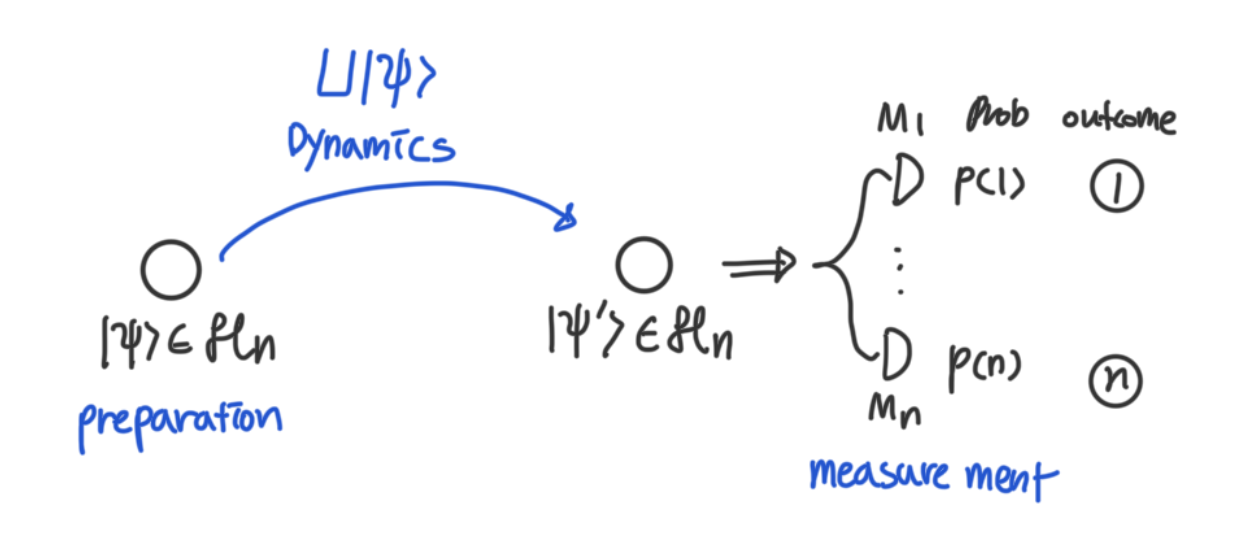
\includegraphics[width=0.55\columnwidth]{image/L1_general_quantum.png}
                    \end{figure}
                \item 양자역학에서 두 실험이 완전히 동등하려면, 다음 조건을 만족해야한다. 
                \begin{itemize}
                    \item 동일한 initializer를 사용한다.
                    \item 동일한 dynamics를 사용한다.
                    \item 동일한 measurement operator set을 사용한다.
                \end{itemize}
            \end{itemize}
            \vspace{0.2cm}
            $\Rightarrow$ 그러나, 양자역학은 동일한 structure를 사용한다고 하더라도 최종 결과로 얻게되는 outcome은 \textit{probability}에 의하여 결정되기 때문에 다를 수 있다!
        \end{frame}

        \begin{frame}
            \frametitle{Components of quantum theory}
            \begin{block}{Components of quantum theory}
                양자역학은 다음의 4가지 component로 이루어진다.
                \begin{itemize}
                    \item State $\ket{\psi}$
                    \item Dynamics $U$
                    \item Measurement $\{M_i\}$
                    \item Observable $O$
                \end{itemize}
            \end{block}
            \vspace{0.2cm}
            \textbf{State}: unit vector in Hilbert space 
            $$ \ket{\psi} \in \mathcal H,\quad \braket{\psi|\psi} = 1.$$
            \vspace{0.2cm}
            \\\textbf{Dynamics}: unitary operator
            $$\ket{\psi_0} \rightarrow \ket{\psi_t} = U_t\ket{\psi_0},$$
            \textit{where} unitary:
            $$ U^\dagger U = UU^\dagger = I \Leftrightarrow U^\dagger = U^{-1}.$$
        \end{frame}

        \begin{frame}
            \frametitle{Components of quantum theory}
            \textbf{Measurement}: POVM(Positive Operator Value Measurement)
            \vspace{0.3cm}
            \begin{itemize}
                \item POVM은 positive이며, completeness relation을 만족하는 measurement operator들의 집합을 의미한다. 
                $$\Big\{M_i \ : \ M_i \ge 0,\ \sum_i M_i = I \Big\}$$
                \item measurement probability: measurement outcome이 $o_i$일 확률은 다음과 같다. 
                $$ p(i) = \braket{\psi | M_i | \psi}$$
                \vspace{0.1cm}

                \checkmark \underline{meaning}: $|\{M_i\}|$개의 detector가 존재할 때, 측정결과가 각 detector $M_i$에서 감지될 확률 $p(i)$를 위와 같이 표현한다고 생각하자.
            \end{itemize}
        \end{frame}


    \begin{frame}
        \frametitle{Components of quantum theory}
        \textbf{Observable}: Hermitian operator
        \vspace{0.3cm}
        \begin{itemize}
            \item Observable은 각 measurement operator와 그 operator에 대응되는 측정결과[$\ast$]의 linear combination으로 정의된다.
            $$ O = \sum_{i}o_i M_i,\quad (o_i \in \mathbb R)$$
            \textit{where} Hermitian[$\ast$]:
            $$ O^\dagger = O.$$
            \vspace{0.1cm}
            \item Observable은 주어진 quantum state $\ket \psi$에서 해당 관측량 $O$에 대한 measurement를 진행했을 때 얻을 수 잆는 outcome의 기댓값과 관계가 있다.
            $$ \underbrace{\braket{o}}_{empirical} = \sum_i o_i p(i) = \sum_i o_i \braket{\psi | M_i| \psi} = \braket{\psi | O | \psi} = \underbrace{\braket{O}_{\psi}}_{true}$$
        \end{itemize}
    \end{frame}
\end{section}


    %#################################### 
    \begin{section}{Quantum experiment: Qubit}
        \begin{frame}
            \frametitle{Overview of qubit system}
            앞으로 quantum experiment를 다룰 때는 양자역학에서 \alert{정보의 단위}; qubit를 사용한다.
            \begin{itemize}
                \item Qubit는 마치 classical bit처럼 $0$, $1$이라는 measurement outcome을 가진다.
                \item 그러나 qubit의 state (vector)는 \textit{superposition} 상태를 가질 수 있다.
                \item Qubit system에서 사용하는 operation structure는 다음과 같다.
                \begin{itemize}
                    \item initializer: single qubit에 대해, 2차원 hilbert space $\mathcal{H}_2$
                    \item dynamics: $2\times 2$ unitary matrix
                    \item bit detector: 0 또는 1을 감지 (projective measurement)
                    
                \end{itemize}
            \end{itemize}
            \vspace{0.1cm}
            \begin{figure}
                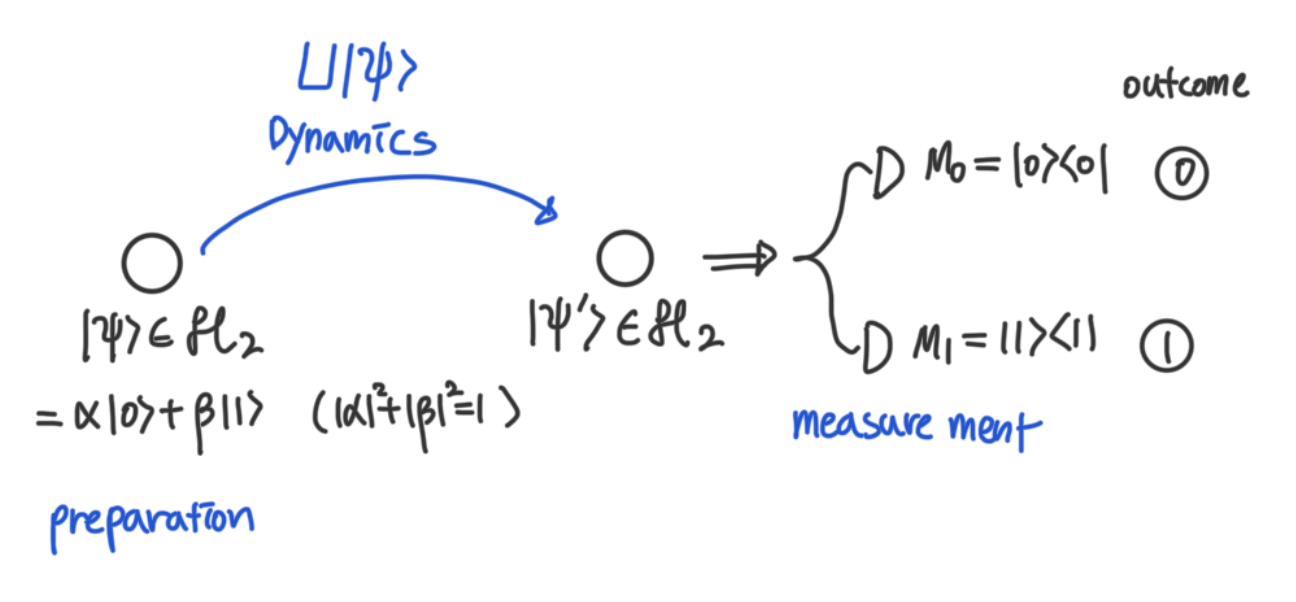
\includegraphics[width=0.6\columnwidth]{image/L1_qubit.png}
            \end{figure}
        \end{frame}

        \begin{frame}
            \frametitle{Qubit state}
                \begin{itemize}
                    \item 2차원 Hilbert space에서 computational basis $\{\ket 0, \ket 1\}$을 사용하면, state를 다음과 같이 표현할 수 있다.
                    $$ \ket{\psi} = \alpha \ket 0 + \beta \ket 1,\qquad \alpha, \beta \in \mathbb C$$
                    \item 이때 각 복소수 계수는 complex exponential을 사용하여 나타낼 수 있다. %!변환과정 직접 써보기
                    ($ \alpha = e^{ia} \cos \frac{\theta}{2}$ $\beta = e^{ib} \sin \frac{\theta}{2}$)
                    \item \textit{Global phase}: 다음 두 상태는 physically 동일하다.
                    $$ \ket \psi = e^{i\phi} \ket \psi$$ 
                    $\ast$ \underline{Proof}:
                    \vspace{0.5cm}

                \end{itemize}
                \begin{definition}[Qubit state]
                    We define state of qubit is two-dimensional vector in the Hilbert space, and we denoted as
                    $$ \begin{aligned} \ket{\psi}  = \alpha \ket{0} + \beta \ket{1} 
                    = \cos  \frac{\theta}{2}  \ket 0+ e^{i \phi} \sin  \frac{\theta}{2}  \ket 1. \end{aligned}$$ 
                    
                \end{definition}
        \end{frame}

        \begin{frame}
            \frametitle{Qubit dynamics}
                주로 사용되는 single qubit dynamics(=gate)는 다음과 같다.
                \begin{itemize}
                    \item Pauli matrices 
                    $$
                    X \triangleq \left(\begin{array}{cc}
                    0 & 1 \\
                    1 & 0
                    \end{array}\right) ; \quad Y \triangleq\left(\begin{array}{cc}
                    0 & -i \\
                    i & 0
                    \end{array}\right); \quad Z \triangleq\left(\begin{array}{cc}
                    1 & 0 \\
                    0 & -1
                    \end{array}\right)
                    $$
                    또한, Pauli matrices는 spectral decomposition으로 표현할 수 있다.
                    \begin{itemize}
                        \item $X = \ket + \bra + - \ket - \bra -$
                        \item $Y = \ket i \bra i - \ket{-i} \bra {-i}$
                        \item $Z = \ket 0 \bra 0 - \ket 1 \bra 1$
                    \end{itemize}
                    \vspace{0.1cm}
                    % $\rightarrow$ 이들은 모두 unitary \& hermitian이므로 observable로 사용할 수 있다. 
                    \item Hadamard gate
                    \vspace{0.05cm}
                    \\ Hadamard gate를 이용하면 $X$ gate와 $Z$ gate를 서로 전환할 수 있다. 
                    $$
                    H \triangleq \frac{1}{\sqrt 2} \left(\begin{array}{cc}
                    1 & 1 \\
                    1 & -1
                    \end{array}\right) 
                    $$ 
                    \item Phase gate
                    $$
                    P(\alpha) \triangleq  \left(\begin{array}{cc}
                    1 & 0 \\
                    0 & e^{i \alpha}
                    \end{array}\right),\qquad (P(\pi) = S,\ P(\pi/8) = T)
                    $$
                \end{itemize}
        \end{frame}

        \begin{frame}
            \frametitle{Example}
            다음 회로들에 대하여, 각 detector에 대한 확률 $p(0), p(1)$을 계산하라. 
            \vspace{0.5cm}
            \begin{columns}
                \begin{column}{0.4\textwidth}
                    \textbf{Example 1}
                    \begin{figure}
                        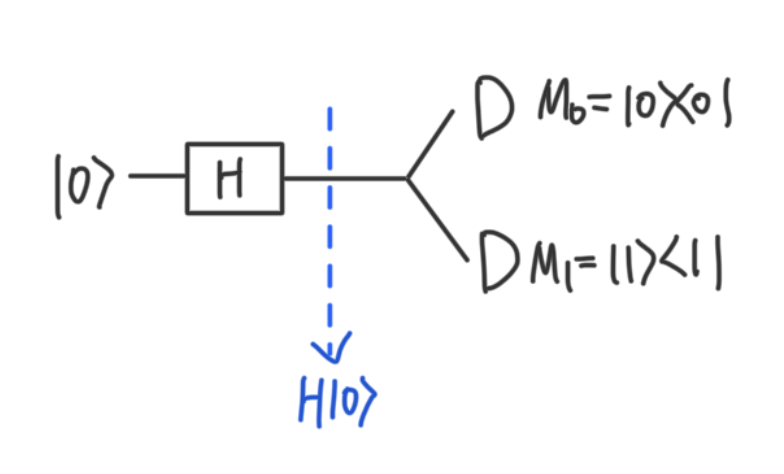
\includegraphics[width=0.8\columnwidth]{image/L1_ex1.png}
                    \end{figure}

                \end{column}

                \begin{column}{0.6\textwidth}
                    \textbf{Example 2}
                    \begin{figure}
                        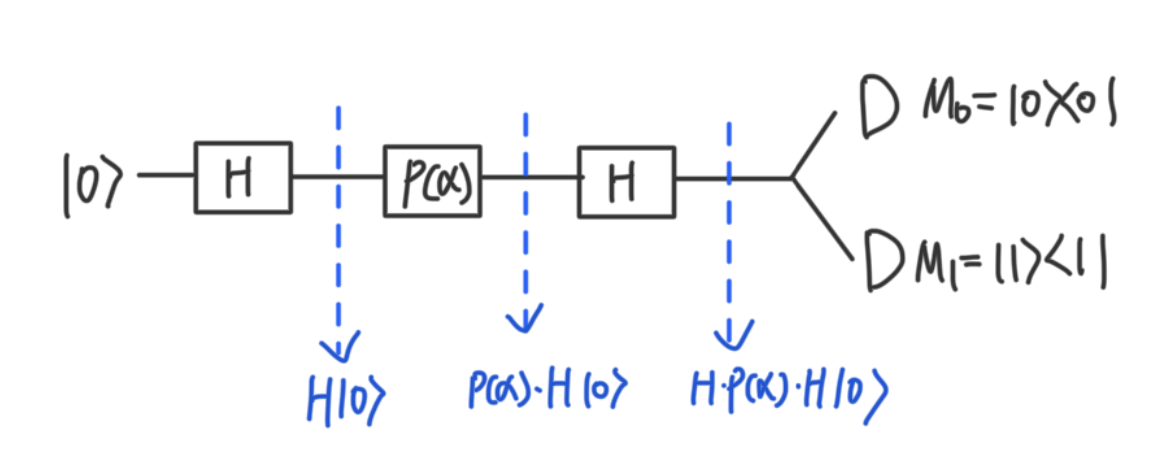
\includegraphics[width=0.8\columnwidth]{image/L1_ex2.png}
                    \end{figure}

                \end{column}
            \end{columns}
            \vspace{0.8cm}
            $\Rightarrow$
            \vspace{2cm}
        \end{frame}
    \end{section}


    %#################################### 
    \begin{section}{Mixed state}
        \begin{frame}
            \frametitle{Prerequisites: trace}
            \begin{definition}[trace]
                Given matrix $A$, \textbf{trace} is a sum of diagonal matrix. On the other hand, it is also a sum of \textit{eigenvalue}.
                $$\begin{aligned} \operatorname{Tr}(A) & = \sum_{i} a_{ii} = \sum_{i} \braket{i|A|i} \\ &= \sum_i \lambda_i \end{aligned}$$
            \end{definition}
            \begin{theorem}[property of trace]
                \begin{itemize}
                    \item $\operatorname{Tr}(AB) = \operatorname{Tr}(BA)$
                    \item $\braket{\psi | A | \psi} = \operatorname{Tr}(A \ket \psi \bra \psi)$
                \end{itemize}
            \end{theorem}
            $\ast$ \underline{Proof}:
            \\$\Rightarrow$
            \vspace{1cm}
        \end{frame}

        \begin{frame}
            \frametitle{Mixed state}
            \begin{itemize}
                \item State를 preparation할 떄, deterministic하게 결정하는 것이 아니라 특정한 확률에 따라서 state를 $\ket{\psi_0}$ 또는 $\ket{\psi_1}$로 준비하는 상황을 가정하자.
                \begin{figure}
                    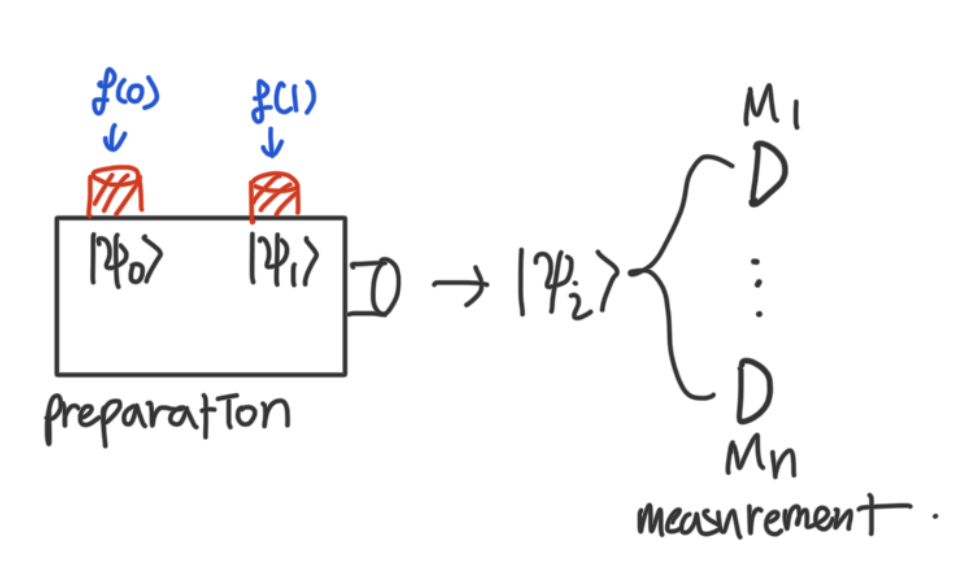
\includegraphics[width=0.4\columnwidth]{image/L1_mixed_experiment.png}
                \end{figure}
                \item 이렇게 결정된 임의의 state $\ket{\psi_i}$에 대하여 outcome이 $o_i$일 확률은 다음과 같다.
                $$ \tilde{p}(i) = q(0) \underbrace{\braket{\psi_0 |M_i| \psi_0}}_{p(i|\psi_0)} + q(1) \underbrace{\braket{\psi_1 |M_i| \psi_1}}_{p(i|\psi_1)} $$
                \textit{by property of trace},
                \begin{align*}\tilde{p}(i) &= q(0) \operatorname{Tr}\big(M_i \ket{\psi_0} \bra{\psi_0}\big) + q(1)\operatorname{Tr}\big( M_i \ket{\psi_1} \bra{\psi_1}\big) \\ &= \operatorname{Tr} \Big(M_i  \big( \underbrace{q(0) \ket {\psi_0} \bra {\psi_0} + q(1) \ket {\psi_1} \bra {\psi_1}}_{state} \big)\Big)\end{align*}
            \end{itemize}
        \end{frame}

        \begin{frame}
            \frametitle{Mixed state}
            \begin{itemize}
                \item 따라서 이처럼 여러가지의 state 후보들이 non-deterministic하게 존재할 때, 그 state를 나타내기 위해서는 다른 표기법을 이용해야한다.
                \item Density matrix를 사용할 때는 measurement와 state의 곱에대한 trace를 계산하여 확률을 구할 수 있다.
                $$p(i) = \operatorname{Tr}(M_i \cdot \rho)$$
            \end{itemize}
            \begin{definition}[density matrix]
                \textbf{Density matrix} is convex combination of pure states. We denoted as:
                $$ \rho = \sum_{i=0}^n q(i) \ket{\psi_i} \bra{\psi_i}$$
                \textit{where} $\ket{\psi_i} \bra{\psi_i}, \forall i$ are pure states.
            \end{definition}
            \begin{theorem}[condition of pure state]
                If $\rho$ is pure state, then if and only if $\operatorname{Tr}(\rho^2) = 1$
            \end{theorem}
        \end{frame}
    \end{section}

    %#################################### 
    \begin{section}{Quantum experiment: aspect of quantum physics}
        \begin{frame}
            \frametitle{Preparation and dynamics with energy}
            \textbf{Preparation}
            \begin{itemize}
                \item qubit의 computational basis $\ket 0, \ket 1$은 system의 \alert{energy level}과 연관된다.
                \item 일반적으로 초기화에 사용하는 $\ket 0$ state가 ground state에서의 energy이다.
                $$\ket{0} \leftrightarrow E_0, \qquad \ket{1} \leftrightarrow E_1,\qquad (E_0 < E_1) $$
            \end{itemize}
            \vspace{0.2cm}
            \textbf{Dynamics}
            \begin{itemize}
                \item state가 energy에 연관되어 있기 때문에, 계의 state를 변화시키기 위해서는 \alert{계의 에너지를 변화}시켜야한다.
                \item 즉, dynamics는 계에 $\Delta E$만큼의 energy변화를 야기시킨다.
            \end{itemize}
            \begin{figure}
                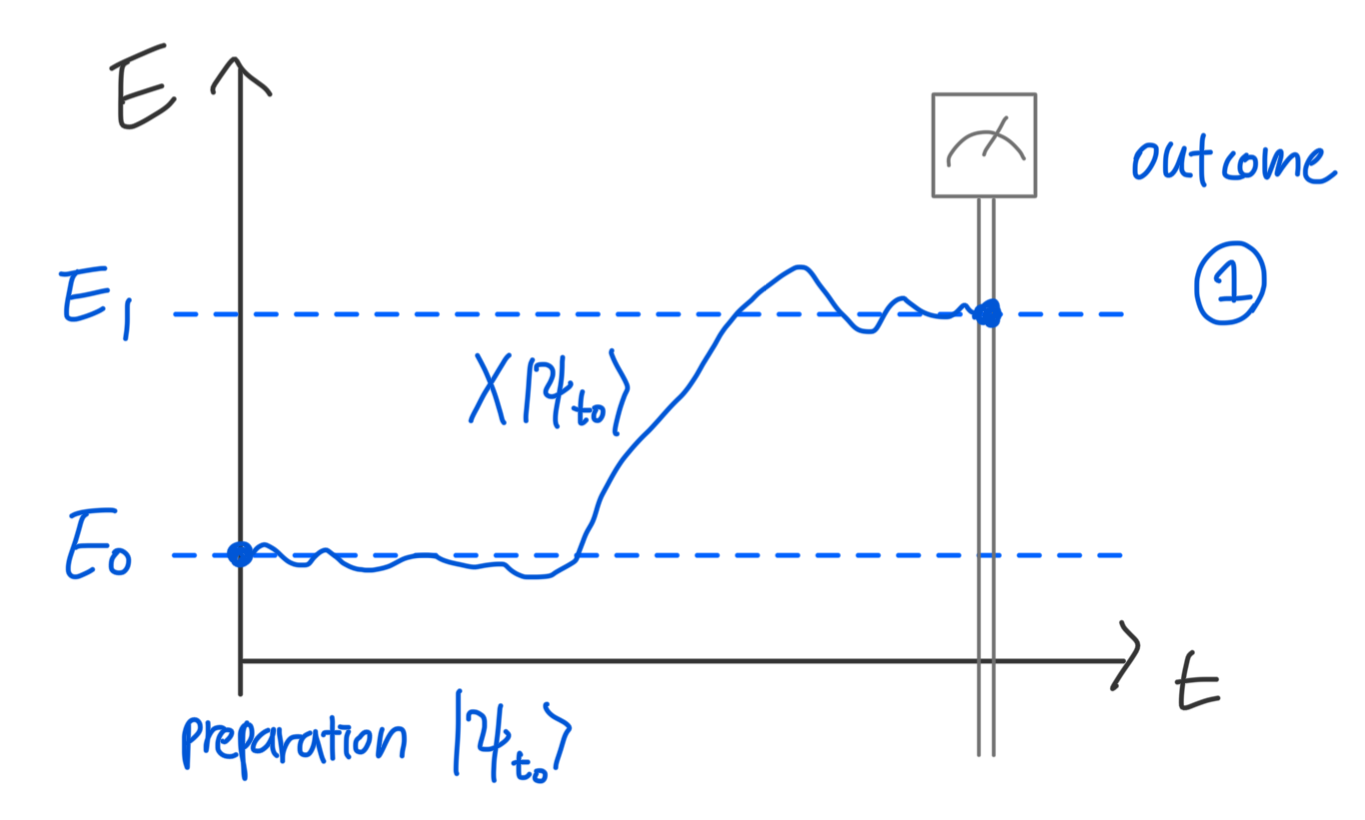
\includegraphics[width=0.45\columnwidth]{image/L1_energy.png}
            \end{figure}
            \vspace{-0.1cm}
        \end{frame}

        \begin{frame}
            \frametitle{Dynamics with Hamiltonian: Schrodinger equation}
            Quantum mechanics에서 \textbf{dynamics}는 Schrödinger equation으로부터 유도할 수 있다.
            \begin{theorem}[time-dependent Schrödinger equation]
                Time-dependent Schrödinger equation:
                $$i \hbar \frac{d}{dt} \ket{\psi(t)} = H\ket{\psi(t)}$$
                \textit{where} $H$ is an observable, the Hamiltonian operator
            \end{theorem}
            \vspace{0.4cm}
            time-dependent Schrödinger equation을 풀면, 시간의 변화에 따른 state의 변화를 다음과 같이 기술할 수 있다.
            \begin{corollary}[time-dependent state transition]
                $$\ket{\psi(t) } = e^{-i H(t-t_0)} \ket{\psi(t_0)}$$
            \end{corollary}
            \checkmark \underline{meaning}: 즉, dynamics는 $e^{-iH(t-t_0)}$이다.
        \end{frame}


        \begin{frame}
            \frametitle{Dynamics with Hamiltonian: Schrodinger equation}
            \begin{itemize}
                \item Hamiltonian 역시 operator이므로 eigenvalue $E_k$, 그리고 eigenvector $\ket{\psi_k}$가 존재하기 때문에, spectral decomposition을 할 수 있다.
                \begin{equation}
                    H = \sum_k E_k \ket{\phi_k} \bra{\phi_k}
                \end{equation}
                \item Hamiltonian의 eigenvector는 Hilbert space의 \textit{eigenbasis}이므로 이를 이용하여 state를 표현할 수 있다.
                \begin{equation}
                    \ket{\psi(t_0)} = \sum_k c_k \ket{\phi_k}
                \end{equation}
                \item Matrix exponential을 이용하여, dynamics를 다음과 같이 전개할 수 있다.
                \begin{equation}
                    e^{-iH(t-t_0)} = \sum^\infty_{n=0} \frac{1}{n!}(-i)^n H^n (t-t_0)^n
                \end{equation}
                \item 그렇다면, $\ket{\psi(t_0)} = \ket{\phi_k}$일 때, $\ket{\psi(t)}$는 다음과 같이 쓸 수 있다.
                \begin{align*}
                    \ket{\psi(t)} = e^{-iH(t-t_0)}\ket{\phi_k} &=^{(3)} \sum^\infty_{n=0} \frac{1}{n!}(-i)^n (t-t_0)^n H^n \ket{\phi_k}   \\ &=^{(1)} \sum^\infty_{n=0} \frac{1}{n!}(-i)^n (t-t_0)^n E_k^n \ket{\phi_k} \\ &=^{(thr)} e^{-iE_k(t-t_0)} \tag{4}\ket{\phi_k} 
                \end{align*}
            \end{itemize}
        \end{frame}

        \begin{frame}
            \frametitle{Dynamics with Hamiltonian: Schrodinger equation}
            Eq 2, 4를 이용하면, 어떤 arbitrary state $\ket{\psi(t_0)}$에 대한 state transition을 다음과 같이 나타낼 수 있다.
            \begin{align*}\ket{\psi(t)} &= e^{-iH(t-t_0)}\ket{\psi(t_0)} \\&= e^{-iH(t-t_0)}\sum_k c_k \ket{\phi_k}\tag{by Eq.2} \\&=\sum_k c_ke^{-iH(t-t_0)} \ket{\phi_k} \\ &=\boxed{\sum_k c_ke^{-iE_k(t-t_0)}\ket{\phi_k}\tag{by Eq.4}}\end{align*}
            
            \vspace{0.5cm}
            따라서 $\ket{\psi(t)}, \ket{\psi(t_0)}$ 모두 $\{\phi_k\}$들의 linear combination으로 표현되므로, 각 basis vector에 대한 coefficient를 변경시켜서 state transition을 만들 수 있다. 이 과정은 unitary matrix를 사용하여 표현된다. ($c_k \rightarrow c_k e^{-i E_k (t-t_0)}$)
            $$\ket{\psi(t)} = U(t, t_0) \ket{\psi(t_0)}$$
            \textit{where} $U(t, t_0) = e^{-iHt}$
        \end{frame}
    \end{section}

    %#################################### 
    \begin{section}{Quantum gate}
        
        \begin{frame}
            \frametitle{Gate with Hamiltonian}
            \begin{itemize}
                \item single qubit system에서 다음의 Hamiltonian을 사용한다고 하자. % (Hermitian) 만족
                $$\ket{\psi} = c_0 \ket0 + c_1 \ket 1,\quad H = \alpha I + \beta X$$
                \item Spectral decomposition으로 $H$를 표현하면, matrix exponential을 구할 수 있다.
                \begin{align*} H &= \alpha(\ket + \bra + + \ket - \bra - ) + \beta(\ket + \bra + - \ket- \bra -) \\ &= (\alpha+ \beta) \ket + \bra + + (\alpha - \beta) \ket - \bra -\end{align*}
                \item 따라서 Hamiltonian에 exponential을 취하면 다음과 같다.
                $$e^{-iHt} = e^{-i\alpha t}[e^{-i\beta t}\ket+ \bra + + e^{i\beta t} \ket - \bra -]$$
                \item Time-dependent Schrödinger equation에 의해, $\ket{\psi(t)}$ state는 다음과 같다.
                \begin{align*}
                    \ket{\psi(t)} &= e^{-iHt} \ket{\psi(0)} = e^{-iHt} (c_0 \ket{0} + c_1 \ket{1}) \\ &=e^{-i\alpha t}[e^{-i\beta t}\ket+ \bra + + e^{i\beta t} \ket - \bra -](c_0 \ket{0} + c_1 \ket{1})\\ 
                    &= e^{-i\alpha t}\left[ e^{-i\beta t}c_0 \frac{1}{\sqrt 2} \ket{+}+e^{i\beta t}c_0 \frac{1}{\sqrt 2} \ket{-}+ \frac{1}{\sqrt 2}e^{-i\beta t}c_1 \ket{+}- \frac{1}{\sqrt 2}e^{i\beta t}c_1 \ket{-}\right] \end{align*}

            \end{itemize}
            
        \end{frame}
        
        \begin{frame}
            \frametitle{Some important gates}
            \textbf{Controlled-Z gate}
            \begin{itemize}
                \item method 1: Hamiltonian
                $$ H_{C(Z)} \triangleq E(I-Z) \otimes I-Z, \qquad (t = {\pi \over {4E}}) $$
                \item method 2: Controlled gate
                $$ C(Z) \triangleq \ket 0 \bra 0 \otimes I + \ket 1 \bra 1 \otimes Z $$
            \end{itemize}
            $\ast$ \underline{Proof}:
            \\$\Rightarrow$
            
            \vspace{1.8cm}
            
            \textbf{Controlled-X gate}
            by Hadamard gate,
            \begin{align*} (I\otimes H) C(Z) (I\otimes H)^\dagger &= \ket 0 \bra 0 \otimes HH^\dagger + \ket 1 \bra 1 \otimes HZH^\dagger\\ &= \ket{0} \bra 0 \otimes I + \ket 1 \bra 1 \otimes X = \boxed{C(X)} \end{align*}
            
            \vspace{-0.8cm}
            
        \end{frame}
    \end{section}

    %#################################### 
    \begin{frame}{References}
        
        \begin{itemize}
            \item Lecture notes for EE547: Introduction to Quantum Information Processing (Fall 2024)
        \end{itemize}
        \vspace{6cm}
    \end{frame}

\end{document}